\chapter{System Intent and Development Philosophy}
\chapterquote{RUDRA is best understood as a layered robot, not as a single program. Each layer has one job and one failure boundary.}{Engineering principle for RUDRAv4}

\section{What RUDRAv4 is}

\RUDRAv{} is a four-wheel rover that uses differential-drive control. It accepts operator commands from a wireless PS2 controller and accepts ROS velocity commands through \topic{/cmd_vel}. It drives four DC motors through two Sabertooth motor controllers. It senses the surrounding space through a YDLIDAR and publishes robot telemetry into ROS 2 for monitoring, visualization, and eventual autonomous navigation.

The current architecture keeps the successful RUDRAv3 split-controller hardware model but replaces the old ROS 1 integration style with ROS 2 bridge nodes running on the NUC. Instead of pushing ROS directly into the microcontrollers, the NUC owns the ROS graph and the microcontrollers exchange compact plain-serial packets with it. This makes the system easier to debug because every boundary can be inspected with a serial terminal or a ROS topic echo.

\begin{figure}[htbp]
\centering
\resizebox{0.95\linewidth}{!}{\begin{tikzpicture}[node distance=9mm and 10mm, every node/.append style={font=\small}]
  \node[rudraHw,text width=24mm] (ps2) {PS2 wireless\\controller};
  \node[rudraHw,text width=24mm,right=of ps2] (uno) {Arduino Uno\\PS2 reader};
  \node[rudraBlock,text width=30mm,right=of uno] (nuc) {Intel NUC\\ROS~2 graph};
  \node[rudraHw,text width=24mm,right=of nuc] (teensy) {Teensy~4.1\\drive interface};
  \node[rudraHw,text width=26mm,right=of teensy] (sabers) {2x Sabertooth\\packet serial};
  \node[rudraHw,text width=20mm,right=of sabers] (motors) {4 drive\\motors};
  \node[rudraHw,text width=24mm,above=of nuc] (lidar) {YDLIDAR G2B\\LaserScan};
  \node[rudraHw,text width=28mm,below=of nuc] (dcdc) {DCDC-USB\\NUC power monitor};

  \draw[rudraArrow] (ps2) -- node[above=0.5]{\scriptsize wireless} (uno);
  \draw[rudraArrow] (uno) -- node[above=0.5]{\scriptsize \cmd{J,...}} (nuc);
  \draw[rudraArrow] (nuc) -- node[above=0.5]{\scriptsize \cmd{D,...}} (teensy);
  \draw[rudraArrow] (teensy) -- node[above=1]{\scriptsize 9600 baud} (sabers);
  \draw[rudraArrow] (sabers) -- (motors);
  \draw[rudraArrow] (lidar) -- node[right]{\scriptsize \topic{/scan}} (nuc);
  \draw[rudraDashed] (dcdc) -- node[right,align=center]{\scriptsize \topic{/rudra/}\\\scriptsize \topic{nuc_battery}} (nuc);
\end{tikzpicture}}
\caption{RUDRAv4 layered control architecture. ROS 2 lives on the NUC; the Uno, Teensy, and DCDC-USB remain hardware interface endpoints.}
\label{fig:system-layered}
\end{figure}

\section{The preserved design ideas}

The hardware baseline is intentionally familiar:

\begin{longtable}{p{0.28\linewidth}p{0.62\linewidth}}
\toprule
Element & Current role in RUDRAv4\\
\midrule
PS2 wireless controller & Human operator input for manual mode and obstacle-guard latch control.\\
Arduino Uno & Reads the PS2 receiver through the vendored PS2X library and publishes a compact serial joystick line.\\
Intel NUC & Runs Ubuntu, ROS 2 Lyrical, bridge nodes, LiDAR driver overlays, localization, RViz networking, and power diagnostics.\\
Teensy 4.1 & Receives final drive packets from the NUC and talks packet serial to both Sabertooth drivers. Optional firmware also emits IMU and wheel odometry telemetry.\\
Dual Sabertooth drivers & Drive the right and left motor sides through packet serial addresses 128 and 129.\\
YDLIDAR G2B & Publishes \topic{/scan} for obstacle guard, RViz, SLAM, and navigation experiments.\\
Mini-Box DCDC-USB & Regulates the dedicated NUC rail and exposes voltage/status telemetry over USB.\\
\bottomrule
\end{longtable}

\section{What changed from the older article}

The older RUDRA article mixed ROS 1, Jetson/Nano discussion, rosserial considerations, and the original firmware strategy. This edition keeps the engineering depth but changes the assumptions to match the current workspace:

\begin{itemize}
  \item The onboard computer is the NUC named \cmd{rudra}; the laptop station is \cmd{aghora}.
  \item The ROS stack is ROS 2 Lyrical and is sourced from \filep{/opt/ros/lyrical/setup.bash}.
  \item The robot workspace is \filep{/home/rudra/Projects/RUDRAv4}.
  \item The YDLIDAR SDK and driver are built in an external overlay at \filep{/home/rudra/ros2_ws}.
  \item The microcontrollers use plain serial instead of ROS serial. The plain serial boundary is deliberately simpler: \cmd{J,...} from Uno to NUC and \cmd{D,...} from NUC to Teensy.
  \item DCDC-USB is not treated as a motor-power device. It is the NUC power rail and is monitored through ROS diagnostics.
\end{itemize}

\section{System-of-systems view}

A rover that moves safely has at least five independent loops:

\begin{enumerate}
  \item \textbf{Human command loop}: PS2 controller to Uno to NUC.
  \item \textbf{Drive command loop}: NUC to Teensy to Sabertooth to motors.
  \item \textbf{Perception loop}: LiDAR to \topic{/scan} to obstacle guard and RViz.
  \item \textbf{State-estimation loop}: encoders and IMU to wheel odometry, raw IMU, EKF, and transforms.
  \item \textbf{Power-health loop}: DCDC-USB voltage readings to battery state and diagnostics.
\end{enumerate}

The important design choice is that the loops are coupled only at intentional points. LiDAR does not directly control the Sabertooth. It modifies the final forward command inside a ROS node. The DCDC monitor does not control the drivetrain. It publishes diagnostics. The Uno does not know about LiDAR. It only sends joystick state and the guard latch. This separation makes RUDRAv4 easier to test, easier to explain, and safer to develop.

\begin{figure}[htbp]
\centering
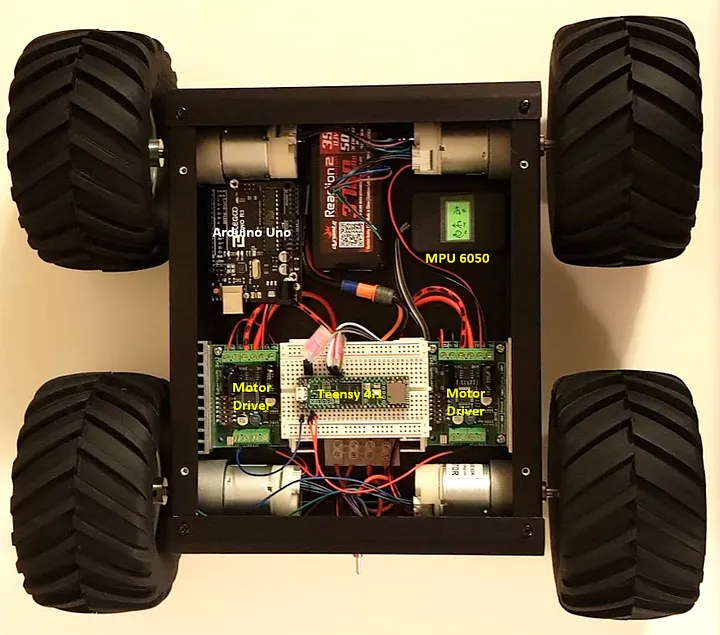
\includegraphics[width=0.72\linewidth]{figures/photos/rudra_chassis_top.png}
\caption{RUDRA chassis and internal electronics. This manual keeps the same modular hardware intent while documenting the current NUC-based RUDRAv4 software stack.}
\end{figure}

\section{Definition of done for the base platform}

For RUDRAv4, a base-control build is considered healthy when the following are all true:

\begin{itemize}
  \item \topic{/rudra/ps2_raw} updates at approximately controller-loop rate when the PS2 controller is active.
  \item \topic{/rudra/drive_cmd} shows only bounded \cmd{D,left,right,enable} lines.
  \item \topic{/rudra/teensy_ack} confirms that the Teensy receives those lines.
  \item \topic{/scan} publishes with frame \cmd{laser} after the YDLIDAR driver starts.
  \item \topic{/rudra/obstacle_guard} changes between clear, slowing, blocked, reverse/turn, disabled, or no-fresh-scan states as expected.
  \item \topic{/rudra/imu/raw}, \topic{/rudra/wheel_odom}, and \topic{/odometry/filtered} publish when localization firmware and launch are used.
  \item \topic{/rudra/nuc_battery} and \topic{/diagnostics} publish when the DCDC monitor is enabled.
  \item RViz on Aghora can view scan, marker, odometry, and transforms on the same DDS domain as Rudra.
\end{itemize}
